\documentclass[11pt]{article}

\usepackage[utf8]{inputenc}
\usepackage[T1]{fontenc}

\usepackage{amssymb}
\usepackage{amsthm}
\usepackage{amsmath}
\usepackage{mathtools}
\usepackage{mathabx}
%\usepackage{framed}
\usepackage{booktabs}
\usepackage{hyperref}
\usepackage{txfonts}
\usepackage{siunitx}
%\usepackage[ngerman]{babel} 

\hypersetup
	{ 
		colorlinks=true,       % false: boxed links; true: colored links
%		hidelinks,
		linkcolor=blue,          % color of internal links (change box color with linkbordercolor)
		citecolor=green,        % color of links to bibliography
		filecolor=magenta,      % color of file links
		urlcolor=cyan,           % color of external links
		linkbordercolor	= {1 0 0},
		citebordercolor	= {0 1 0},	
		urlbordercolor	= {0 1 1}
	}


\usepackage{fontspec}
%\setmainfont{Clear Sans}
%\newfontfamily{\clearsans}{Clear Sans}

\newcommand{\definition}{\\ \textbf{Definition:} \hspace{1cm} }

\newcommand*{\QEDA}{\hfill\ensuremath{\blacksquare}}%
\newcommand*{\QEDB}{\hfill\ensuremath{\square}}%


\begin{document}
	\title{Experimental Physik II Kapitel 15}
		\author
		{
			author\\
			{\small 	\texttt{email}}
		}
		\date{\today}
	\maketitle
	\tableofcontents
	\setcounter{section}{14} %Hier fängt die Nummerierung an.
	
	\newpage
	
\section{Stationäre El. Ströme }
	
	\subsection{}
	\addcontentsline{toc}{subsubsection}{Definition: Elektrischer Strom}
		\textbf{Definition:} \hspace{1cm} Elektrischer Strom := Bewegung von el. Ladung \\
		\\
		Stromst\"{a}rke $\textbf{I} = \frac{dQ}{dt}$ [I] =[$\frac{Ladung}{Zeit}$] $=\dfrac{C}{s} = A$ \\
		Stationäre Ströme: Keine explizite Zeitabhängigkeit.\\ 
		\\
	\addcontentsline{toc}{subsubsection}{Definition: El. Stromdichte}
		\textbf{Definition:} \hspace{1cm} El. Stromdichte \textbf{j} \\
		$j:=\frac{Ladung}{Zeit\cdot Flaeche} $ [$j$] $=\dfrac{A}{m^2}$ \\
		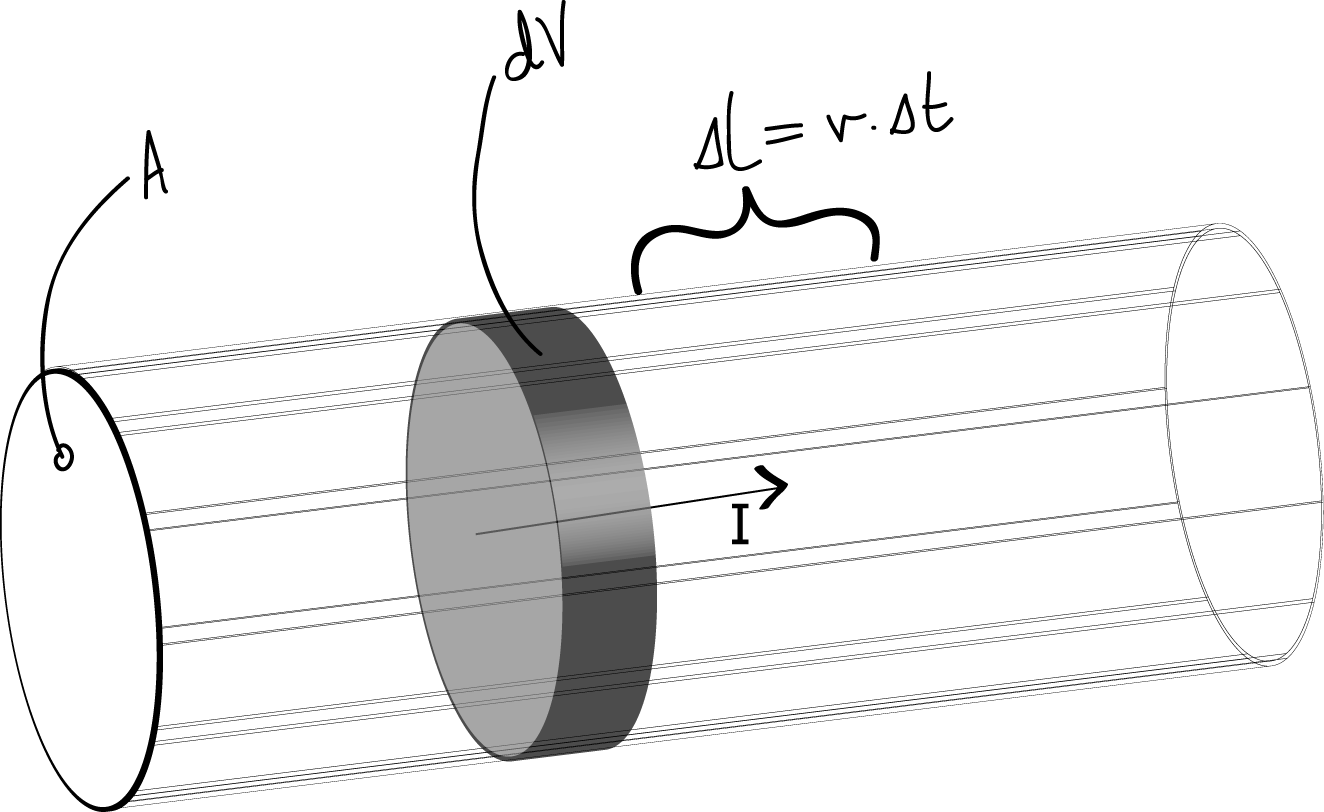
\includegraphics[width=0.6\linewidth]{skizzen/15/VL06/15_1}
		\\
		
		\noindent$N=n\cdot \Delta V $ Ladungsträger \marginpar{($n$ ist die Ladungsträgerdichte)} mit der Ladung q treten im Zeitintervall $\Delta t$ durch $\diameter$-Fläche A. \\
		\\
		Annahme: Alle Ladungen haben die gleiche Geschwindigkeit \emph{v}, dann ist die transportierte Ladung:
		$$\Delta Q=N\cdot q = n\cdot \Delta V \cdot q = n\cdot q \cdot A \cdot \Delta l = n \cdot q\cdot A\cdot v \cdot \Delta t$$
		$$j=\frac{\Delta Q}{\Delta t \cdot A}=n\cdot q \cdot v =  \rho \cdot v $$ \begin{flushright}
			$\rho$ := Ladungsdichte [$C/m^3$]
		\end{flushright}
		{\large \textbf{Allgemein: } \boxed{\vec{j} = \rho \cdot \vec{v} }} \\
		\newpage
		Stromdichte $\longrightarrow$  Stromstärke: $I = {\displaystyle \int\limits_A} \vec J \cdot \mathrm d\vec A$ \\
		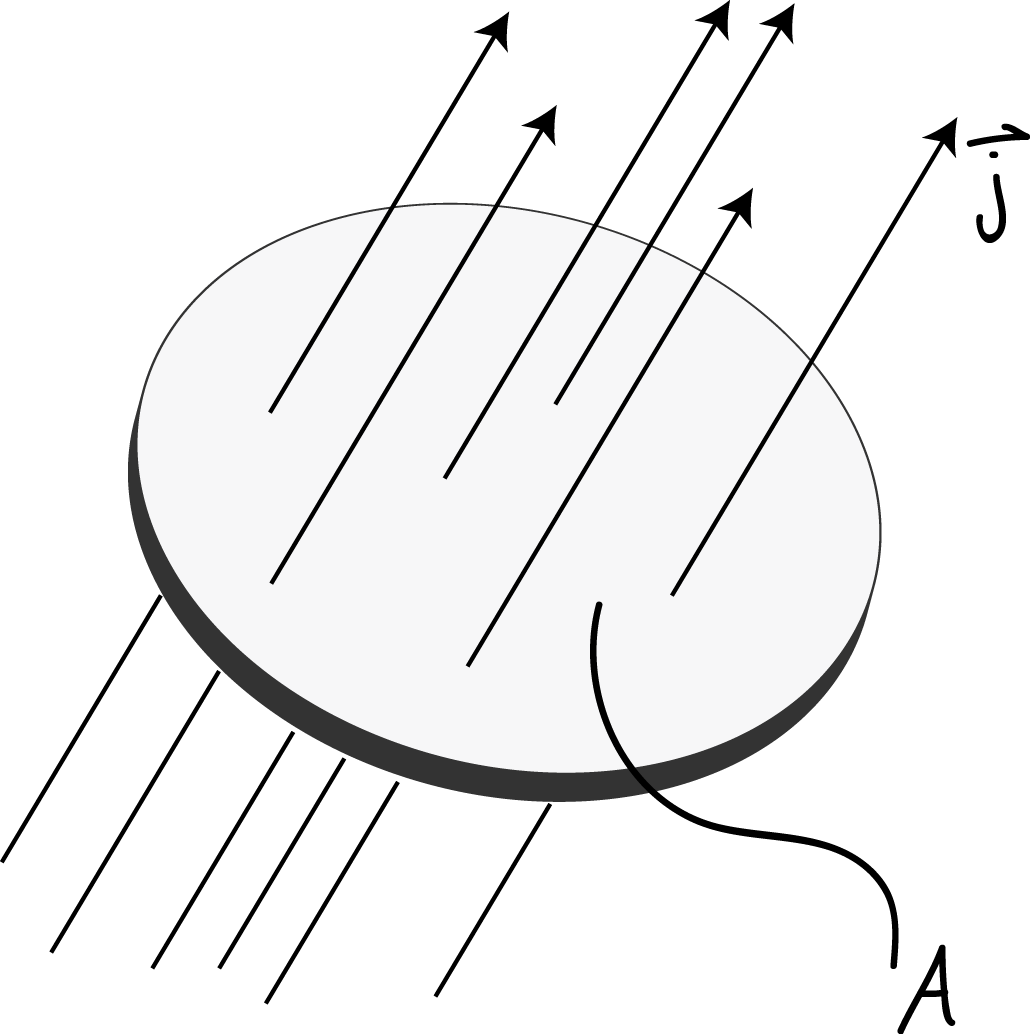
\includegraphics[width=0.3\linewidth]{skizzen/15/VL06/15_2} \\
		\phantomsection
		\addcontentsline{toc}{subsubsection}{Kontinuitätsgleichung}
		\paragraph{\underline{Kontinuitätsgleichung:}}
		Geschlossene Fläche \emph{A} umschließt Volumen \emph{V}.
		$$\underline{I = {\displaystyle\oint\limits_A} \vec{j} d\vec{A} = -\frac{dQ}{dt} = -\frac{d}{dt} \overbrace{{\displaystyle\int\limits_V} \rho \hspace{1mm} dV}^{=Q} }$$
		Differenz zwischen ein. und ausgeströmter Ladung entspricht der negativen Änder der Gesamtladung im Volumen! \\
		($\Rightarrow$ Ladungserhaltung) \\
		\rule{\textwidth}{0.2mm}
		\subsection{Das Ohmsche Gesetz}
		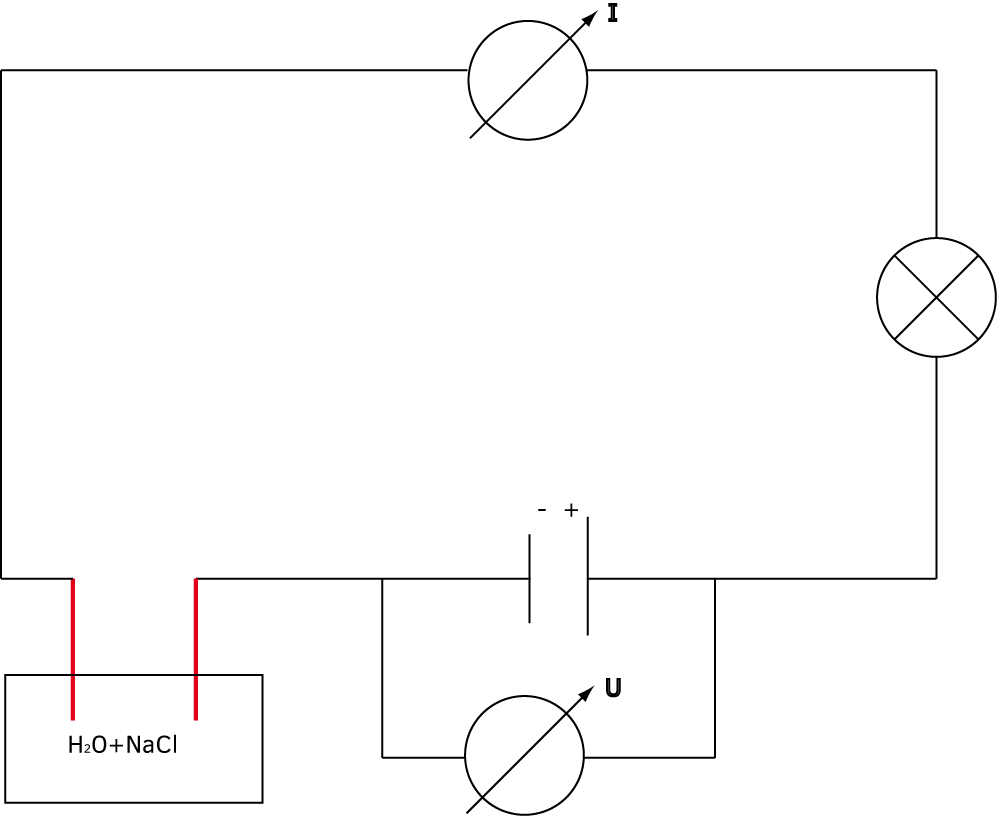
\includegraphics[width=0.7\linewidth]{skizzen/15/VL06/15_3} \\
		$\Rightarrow$ freie Ladungsträger (Ionen) notwendig, damit Strom fließt. \\
		$\Rightarrow$ Dissoziation von $NaCl$ in $Na^+$ und $Cl^-$ \\
		Coulombkraft $|\vec{F_c}| = \frac{1}{4\pi\epsilon_0} \cdot \frac{q_1 \cdot q_2}{r^2} \cdot \frac{1}{\epsilon}$ \\
		$\epsilon_{H_2O}\approx 80 \Rightarrow$ Reduktion von $F_c$ in $H_2o$\\
		\begin{center}
			$\Rightarrow$ \underline{Dissoziation möglich!}
		\end{center}
		qualtitatv: $I \sim U$ \\
		Ersetze Elektrolyt durch Metallwiederstand! \\
		$$I\propto U$$
		\\
		\paragraph{Ohmsches Gesetz:} Wird eine Potenzialdifferenz U and das Ende eines el. Leiters appliziert, so fließt ein el. Strom \emph{I}, dessen Stromstärke proportional zu \emph{U} ist. \\
		{\large $$\boxed{ I = \frac{1}{R} \cdot U }$$} \\
		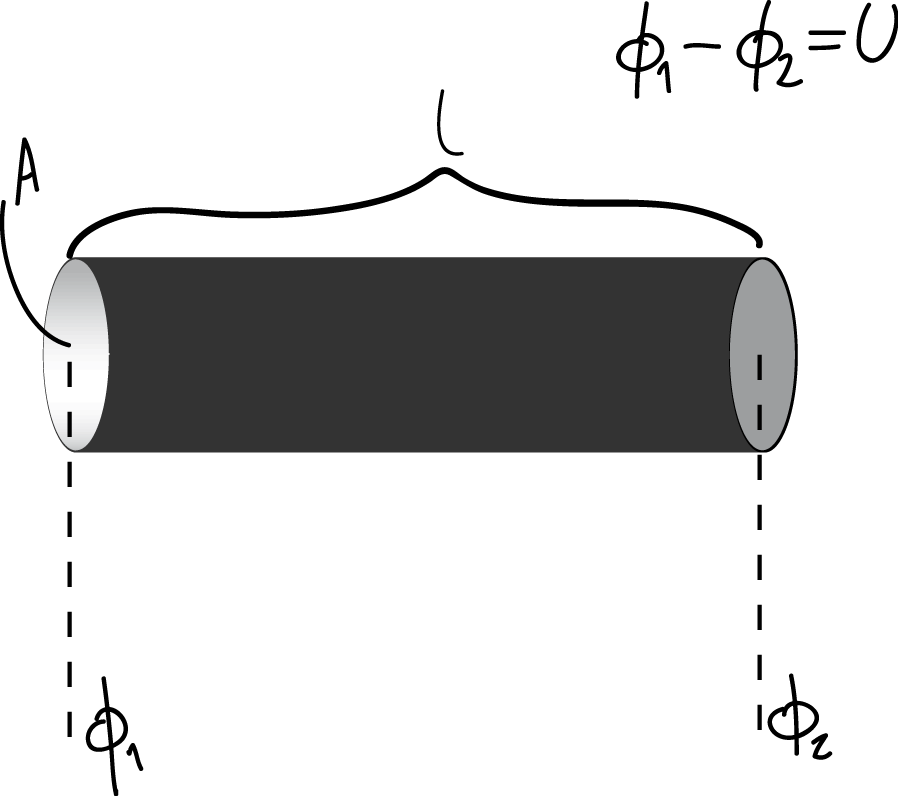
\includegraphics[width=0.8\linewidth]{skizzen/15/VL06/15_4} \\
		Empirischer Befund:
		\begin{align*}
		I &\sim (\phi_2-\phi_1) \\
		I &=\frac{1}{R} (\phi_2-\phi_1) \\
		&= \frac{A}{l} \cdot \frac{1}{\rho} (\phi_2-\phi_1)
		\end{align*}
		
		\noindent \definition $\boxed{R:= \rho \cdot \frac{l}{A}}$ el. Widerstand [\emph{R}] $= \frac{V}{A} = \Omega =$ 1 Ohm \\
		$\rho$: Materialkonstante: spezifischer el. Widerstand [$\rho$] $=\Omega m$ \\
		$\frac{l}{A}$: Geometrieparameter \\
		{\large Ohmsches Gesetz: $\boxed{I=\frac{U}{R}}$} \\
		$\frac{I}{A}=\frac{1}{\rho }\cdot \frac{{\varphi }_{2}-{\varphi }_{1}}{l}$ \\
		$\left|\vec{j}\right|=\frac{1}{\rho }\cdot \left|\vec{E}\right|$ \hspace{2cm} $\frac{1}{\rho} = \sigma := $ el. Leitfähigkeit [$\sigma$] = $Ohm^{-1} m^{-1} = \frac{A}{Vm}$ \\
		$|\vec{j}| = \sigma \cdot |\vec{E}|$ \\
		Empirischer Befund: $\boxed{\vec{j_m} = \sigma_{mn} \vec{E_n} }$ Allegemeines Ohmsches Gesetz\\
		\newpage
		\noindent Mikroskopische betrachtung - Drende Modell \\
		Metall: positiv geladene Atomrümpfe; Elektronen dazwischen beweglich. \\
		
		a.) ohne potenzialdifferenz: thermische ungeorndete bewegung.\\
		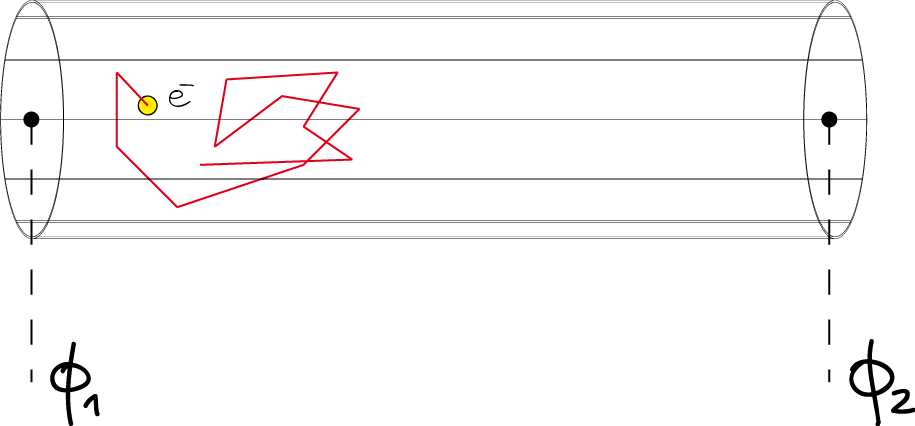
\includegraphics[width=10cm]{skizzen/15/VL06/15_5} \\
		\break
		$ <\vec{v}> = 0 \Rightarrow  $ Im Mittel kein Transport\\
		\begin{align*}
		\text{obwohl: } \sqrt{<v^2>} = \frac{\sqrt{3 K_BT}}{m_e} &\approx 10^5 \frac{m}{s} \\
		&\text{bei } (T=RT) 
		\end{align*}
		b.) $ \phi_2 - \phi_1 \neq 0 \Rightarrow $ El. Feld im Leiter \\
		Zwischen Stößen Beschleunigt durch el. Feld: \\
		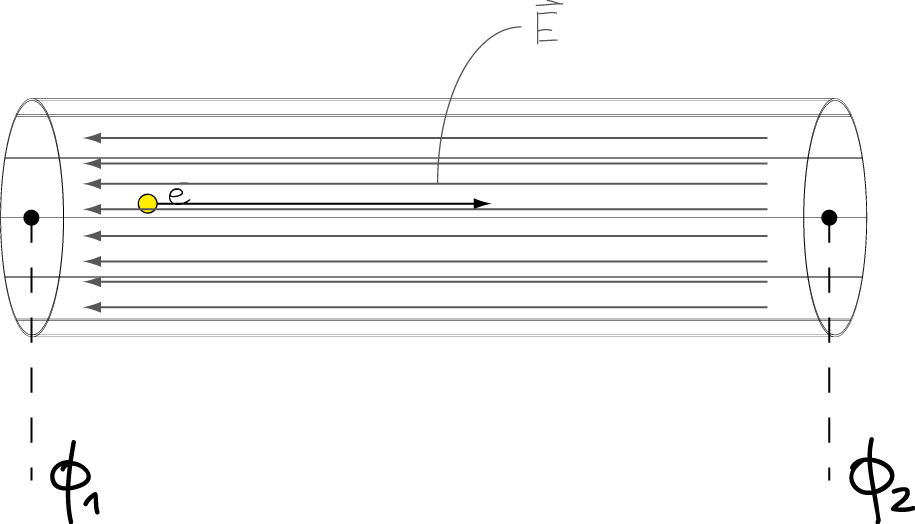
\includegraphics[width=10cm]{skizzen/15/VL06/15_6}\\
		\break
		$\Rightarrow$ \emph{"Drift"} mit Geschwindigkeit $v_D$, die der thermischen Bewegung überlagert ist. \\
		\begin{flalign*}
		\text{Kraft auf Elektron: } \vec{F} &= q_{el} \cdot \vec{E}&&\\
		\Rightarrow \vec{a} &= \frac{q_{el}}{m} \cdot \vec{E}&& \\
		\Rightarrow \vec{v_D} &= \frac{q_{el}}{m} \cdot \vec{E} \cdot \Delta t&& \\
		\end{flalign*} 
		\begin{flalign*}
		\text{ Betrachte Ohmsches Gesetz. } &&\\
		\vec{j} = \sigma \cdot \vec{E} ; \vec{j} = q_{el} \cdot n \cdot \vec{v_D}&& \\
		\text{\underline{Beträge:} } j = \frac{q_{el} \cdot n \cdot v_D}{E} \cdot E = \sigma \cdot E&& \\
		\Rightarrow \sigma = \frac{n\cdot q_{el} \cdot v_D}{E} = const.&& \\
		\Rightarrow \frac{|\vec{v_D}|}{|\vec{E}|} = const.&& \\ 
		\end{flalign*}
		$ |\vec{v_D}|=\mu \cdot |\vec{E}| $ \hspace{1cm} $ \mu $: Beweglichkeit (unabh. von $ \vec{E} $)! \\
		$$ \boxed{\sigma = n\cdot q_{el} \cdot \mu  } $$
		\begin{center}
			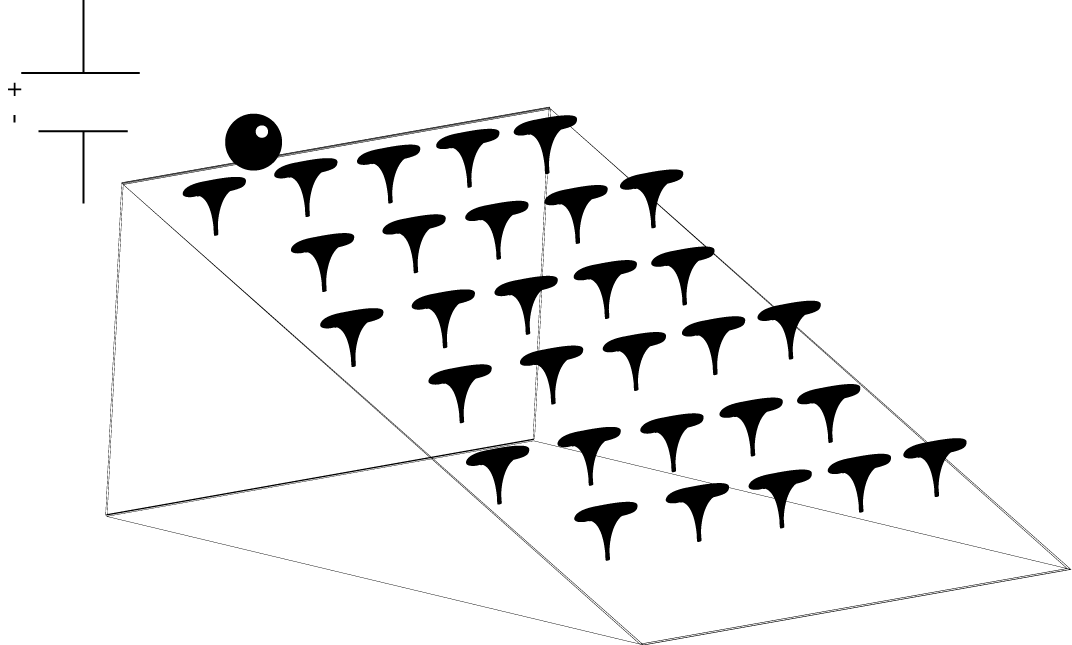
\includegraphics[width=0.5\linewidth]{skizzen/15/VL06/15_7}
		\end{center}
		Damit sich im el. Feld ein Konstates $ v_D $ einstellt, muss es etwas geben\marginpar {$ \Rightarrow $Exp.Phy.I: Stokes-Reibung} wie geschwindigkeitsabhängige Reibung! \\
		$ \Rightarrow $ Makroskopisch: (1-dim) \\
		$$ m\ddot{x}+\frac{m}{\tau}\dot{x} = q_{el}E$$
		$$\boxed{\dot{x} =\frac{q_{el}}{m} \cdot E \cdot \tau \cdot (1-exp(-t/t))}$$
		$ \tau $; Relaxationszeit: Gibt an, nach welcher Zeit \emph{v} auf \emph{v/e} abgenommen hat. \\
		$ \Rightarrow $ \underline{Mikroskopisch:} \\
		$ \tau $: Zeit zwischen zwei Stößen ("Stößzeit") \\
		
		\begin{align*}
		\Rightarrow m \cdot \vec{v_D} = q_{el} \cdot \vec{E} \cdot \tau \\
		\Rightarrow \vec{j} = n\cdot q_{el} \cdot \vec{v_D} = \underbracket[0.5pt][7pt]{\frac{n \cdot q_{el}^2 \cdot \tau}{m}}_{\boxed{\underset{\text{Drude-Leitfähigkeit}}{\sigma = \frac{n \cdot q_{el}^2 \cdot \tau}{m}}}} \cdot \vec{E}\\
		\Rightarrow \boxed{\mu = \frac{q_{el}\cdot \tau}{m}} \hspace{1cm} \text{[$\mu$]} = \frac{m^2}{Vs}
		\end{align*}
		$ \Rightarrow $ Voraussetzung für Gültigkeit des Ohmschen Gesetz:
		\begin{enumerate}
			\item Transport durch Stöße dominiert
			\item \emph{n} unabhängig von $ \vec{E} $
			\item $ \tau $ unabhängig von $ \vec{E} $
		\end{enumerate}
		$ \tau $ klein $\Rightarrow$ $ v_D $ klein (und beobachtbar!) 
		\newpage
		
	\subsection{}
%	\phantomsection
	\addcontentsline{toc}{subsubsection}{(i) Leitung in Elektrolyten}
	\subsubsection*{(i) \underline{Leitung in Elektrolyten}}
	\begin{itemize}
		\item Stofftransport (Ionen) und Ablagerung an Kontakten (Elektroden)
		\item geringe Beweglichkeit
		\item geringe Ladunsträgerkonzentration
	\end{itemize}
	\phantomsection
	\addcontentsline{toc}{subsubsection}{(ii) Leitung in Metallen}
	\subsubsection*{(i) \underline{Leitung in Metallen}}
	\begin{itemize}
		\item Ladungstransport \underline{nur} durch Elektronen
		\item Jedes Atom gibt 1 Elektron ab $ \Rightarrow $ hohe Ladungsträgerdichte (LT)
		\item Beispiel: \begin{align*}
		\text{ Cu, }\hspace{1cm} n &= 8,4 \cdot 10^{28} Ladungen/m^3 \\
		&=8,4 \cdot 10^{22} Ladungen/cm^3
		\end{align*} 
		\item Beweglichkeit: \begin{align*}
		\mu = \frac{\sigma}{n \cdot q} &= \frac{5\cdot10^7(\Omega m)^{-1}}{8,4\cdot 10^{28}m^{-3}\cdot 1,6\cdot 10^{-19}C } \\
		&= 4\cdot 10^{-3} \frac{m^2}{Vs} = 40 \frac{cm^2}{Vs}
		\end{align*}
	\end{itemize}
	\break
	\noindent $ |\vec{E}| ? $ \\
	\begin{align*}
	|\vec{j_{max}}| \approx \frac{5A}{mm^2} &=5\cdot 0^6 A/m^2 \\
	|\vec{E_{max}}| = \frac{|\vec{j_{max}}|}{\sigma} &= 0,1 V/m \\
	<v_D> = \mu |\vec{E}| &= 4\cdot 10^{-4} m/s \approx 0,4 \frac{mm}{s}
	\end{align*}
	$$<v_D> \ll v_ {therm} \text{(ähnlich wie Elektrolyt)}$$
	$$ \tau = \mu \cdot \frac{m}{q} = \underline{2,3 \cdot 10^{-14}s}$$
	Hauptunterschied Metall/Elektrolyt: $ \mu , n $ ! \\
	\begin{flalign*}
	\text{Mittlere freie Weglänge: }  \lambda = v_{therm} \cdot\tau &= 10^5 m/s \cdot \tau &&\\
	&= 20\cdot 10^{-10}m \\
	&= 20 \si{\angstrom}
	\end{flalign*}
	$ \Rightarrow $ca. 20 Atomdistanzen zw. zwei Stößen! 
	\begin{center}
		\rule{5cm}{0.2mm}
	\end{center}
	\noindent Temperaturabhängigkeit: \\
	In el. Leitern gilt: $ R = R(T) $ \\
	Fe-Widerstand:\\
	Abkühlen auf $ LN_2 $-Temp: $ I\longrightarrow I\times2 $\\
	Aufheizen mit Brenner : $  I \longrightarrow I/2 $ \\
	Konstantandraht (Legierung): nahezu keine Änderung \\
	\emph{n} sei temperaturunabhängig!
	$ \Rightarrow T\textuparrow \Rightarrow \tau\textdownarrow,\sigma\textdownarrow $: \\
	Durch thermische Anregung mehr Gitterschwingungen; mehr Stöße! ($ \Rightarrow $Kürzere Stoßzeit) \\
	Konstantan-Legierung: Streuung vornehmlich an Fremdatomen deren Dichte ist T-unabhängig!
	\phantomsection
	\addcontentsline{toc}{subsubsection}{(iii) Leitung in Halbleitern}
	\paragraph{(iii) \underline{Leitung in Halbleitern}} \hfill 
	\break
	\break
	\indent $ T\textuparrow $\hspace{1cm}:\hspace{1cm}$ \sigma \textuparrow $ \\
	Grund:\\
	\indent Starke Temp.-abhängigkeit von n durch thermische Anregung von Ladunsträgern über eine Energielücke \\
	\indent Erhöhung und Kontrolle von $ \sigma $ durch Einbringen von Fremdatomen in Konzentration von $  10 ^{15}cm^{-3}...10^{20}cm^{-3} $: \underline{Dotierung} \\
	$ \Rightarrow \tau $ nimmt auch mit zunehmender \emph{T} ab, aber Zunahme von \emph{n} überwiegt!
	\phantomsection
	\addcontentsline{toc}{subsubsection}{(iv) Leitung im Vakuum}
	\subsubsection*{(iv) \underline{Leitung im Vakuum}} \hfill \break
	Leitung im wesentlichen durch freie Elektronen.\\
	El- Feld zur Beschleunigung $ \Rightarrow $ Ladungstransport\\
	\break
	Erzeugung von freien Elektronen: \\
	\begin{center}
		\begin{tabular}{ c | c  }
			U [V] & I [mA] \\ \hline
			20 & 0,25 \\
			40 & 0,5 \\
			60 & 0,75 \\
			80 & 1,05 \\
			100 & 1,3 \\
			120 & 1,6 \\
			140 & 1,9 \\
			160 & 2,15 \\
			180 & 2,35 \\
			200 & 2,5 \\
			220 & 2,6 \\
			240 & 2,65 \\
			260 & 2,7 \\
			280 & 2,75 \\
			300 & 2,7 \\
		\end{tabular}
	\end{center}
	
	\begin{center}
		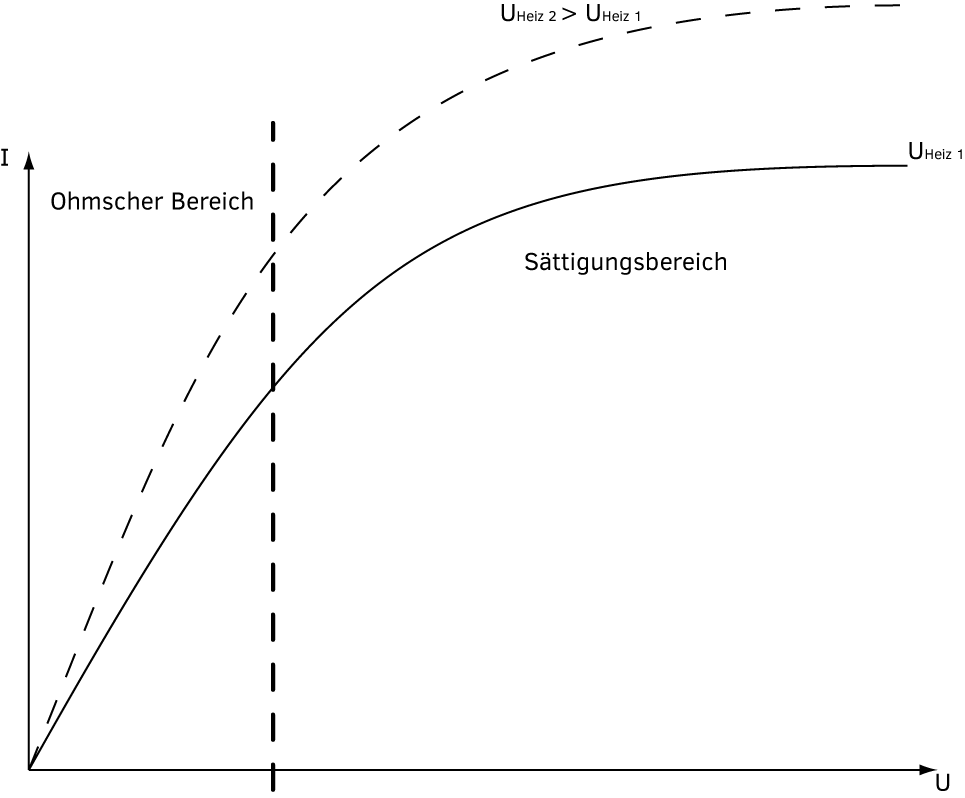
\includegraphics[width=0.8\linewidth]{skizzen/15/VL07/VL7_1.png}
	\end{center}

	$ \Rightarrow $ Umkehrung der Beschleunigungsspannung: Kein Strom! \\
	\newpage
	\noindent Diode:\\
	\begin{center}
		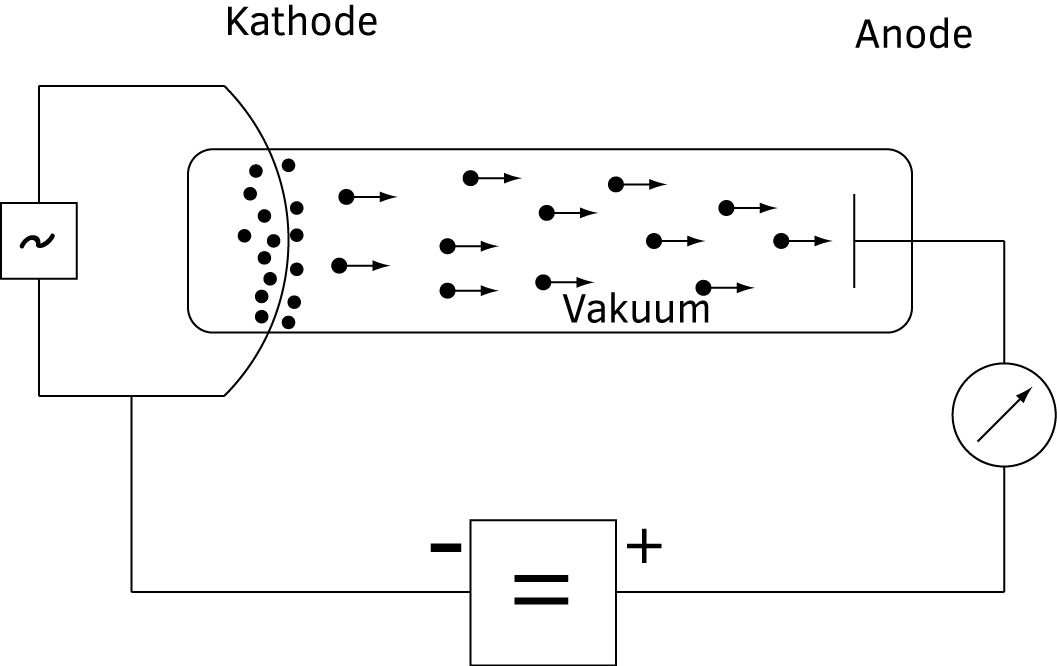
\includegraphics[width=0.7\linewidth]{skizzen/15/VL07/1}
	\end{center}
	 Triode: \\
	\begin{center}
		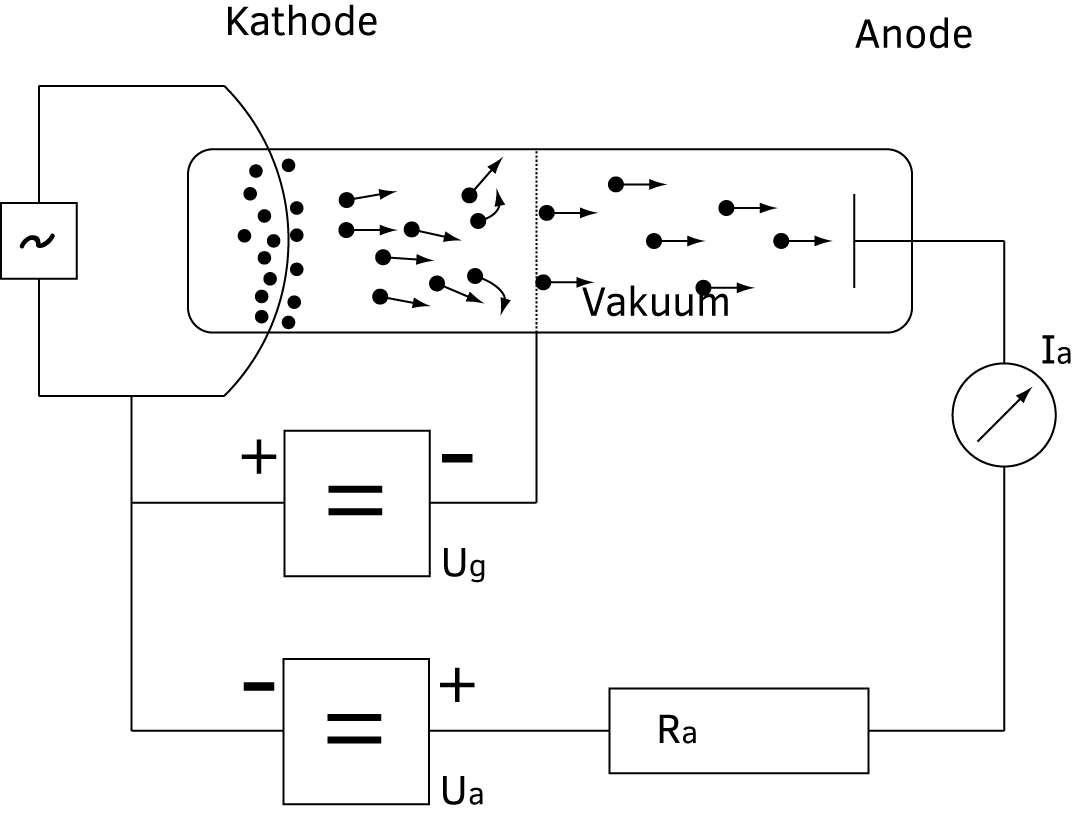
\includegraphics[width=0.7\linewidth]{skizzen/15/VL07/2}
	\end{center}
	\indent $ \Rightarrow $ Verstärkerschaltung möglich!\\
	\phantomsection
	\addcontentsline{toc}{subsubsection}{(v) Leitung in Gasen}
	\subsubsection*{(v) Leitung in Gasen}
	\begin{itemize}
		\item Alle Gase haben sehr kleine Leitfähigkeit\\ ($ \longrightarrow $Entladung des Kondesators an Atmosphäre) \\ ($ \longrightarrow $Gasentladung)
		\item Ladungsträger müssen erzeugt werden: Elektronen, Ionen\\
		Ionisation ist mäglich druch:\\
		\indent Ionisierende Strahlung; Stoßionisation
	\end{itemize}
		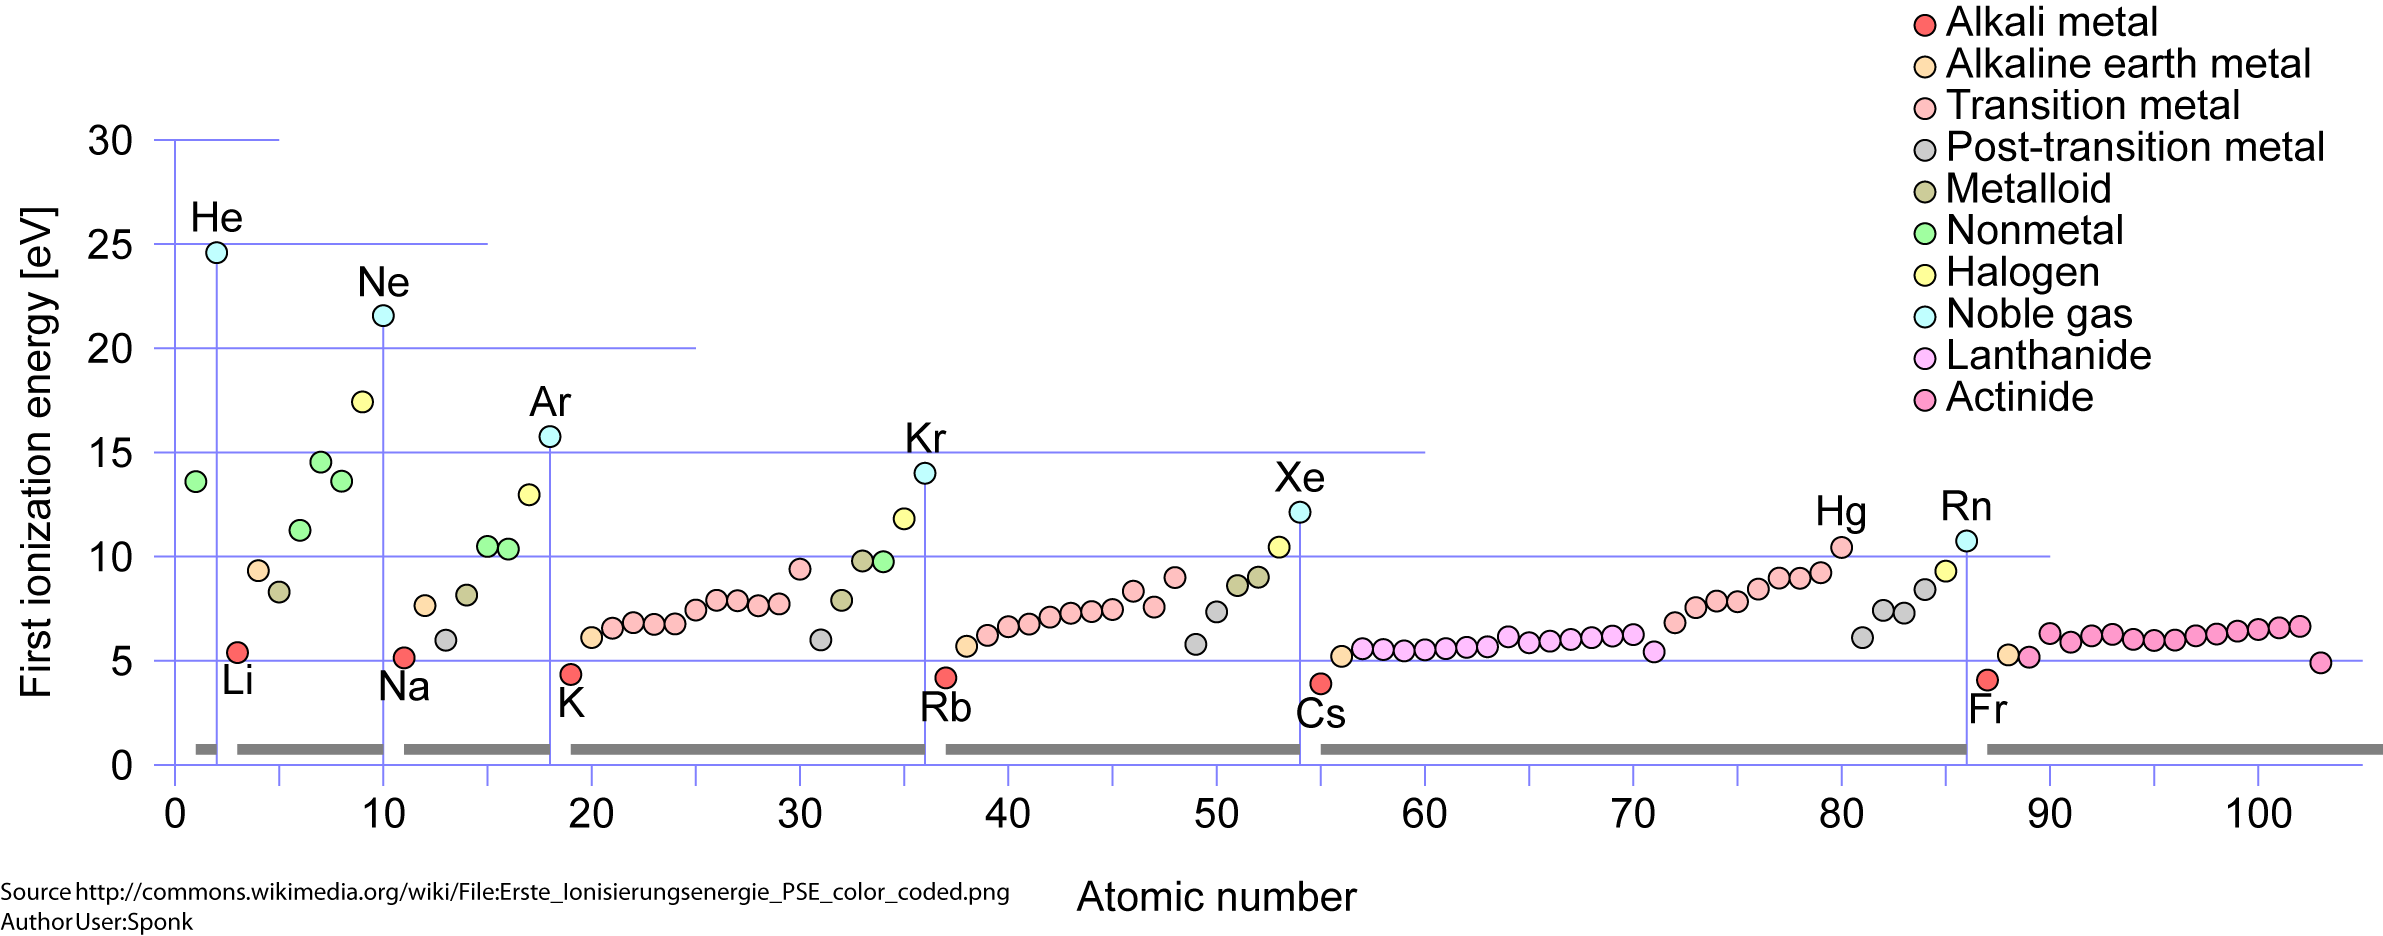
\includegraphics[width=\linewidth]{skizzen/15/VL07/3}\\
	Ionisation braucht Energie!\hfill \break
	Stoßionisation:\\ 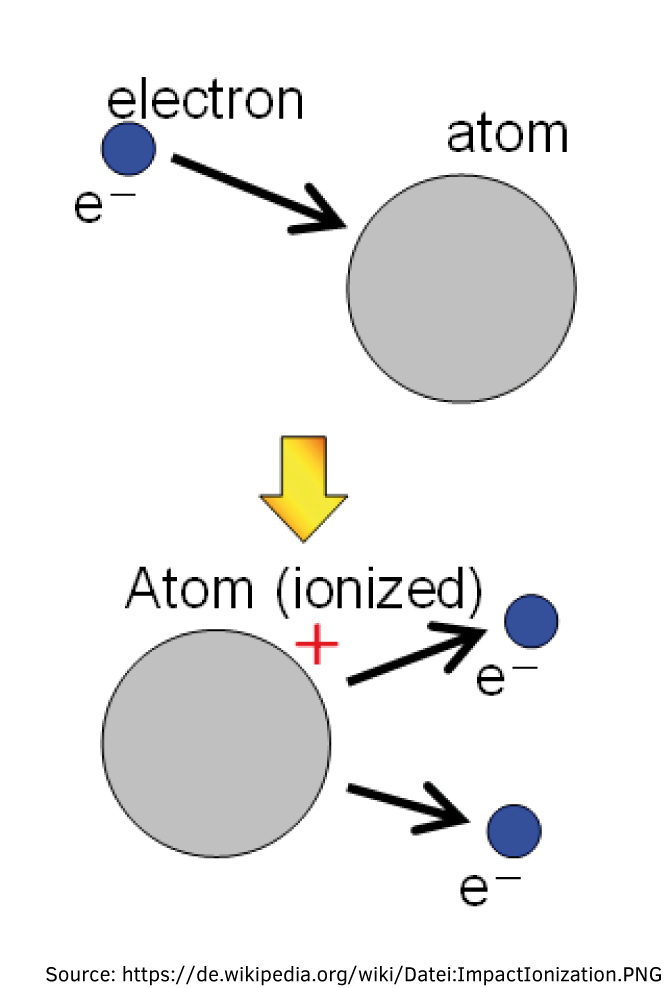
\includegraphics[width=0.5\linewidth]{skizzen/15/VL07/4} \hfill \break
	\newpage \noindent Photoionisation: \\ 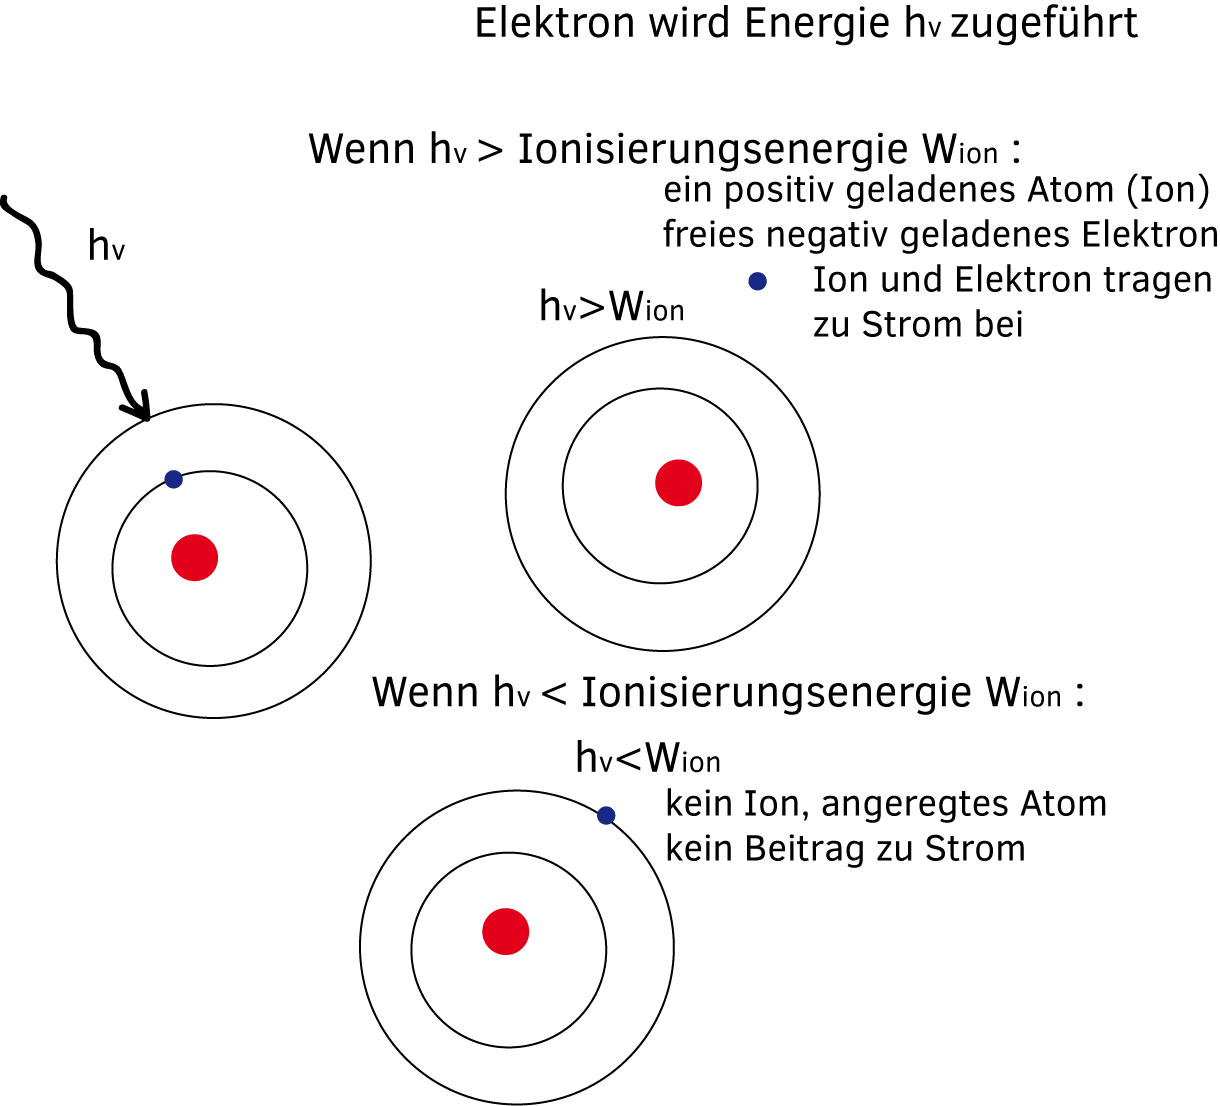
\includegraphics[width=0.7\linewidth]{skizzen/15/VL07/5} \hfill \break
%Thermische Ionisation. \\ \includegraphics[width=0.7\linewidth]{Skizzen/VL07/6} \hfill
	\begin{itemize}
		\item Thermische Ionisation ist möglich.
		\item Glüemission ist auch möglich; Radioaktivität $  \Rightarrow $ ionisierende Strahlung
		\item Rekombination von Ionen und Elektronen ist möglich
	\end{itemize}
	Strom: $ \boxed{I = \underbracket{N}_{\text{\#LT (sehr klein)}} \cdot \overbrace{z \cdot e}^{\text{Ladung: }z \in \mathbb{N} } \cdot \underbrace{\mu}_{ \mu_{\text{Flüssigkeit}} <\mu<\mu_{\text{Metalle}} } \cdot |\vec{E}| } $ \\
	\newpage
	Prinzipieller Aufbau: \\
		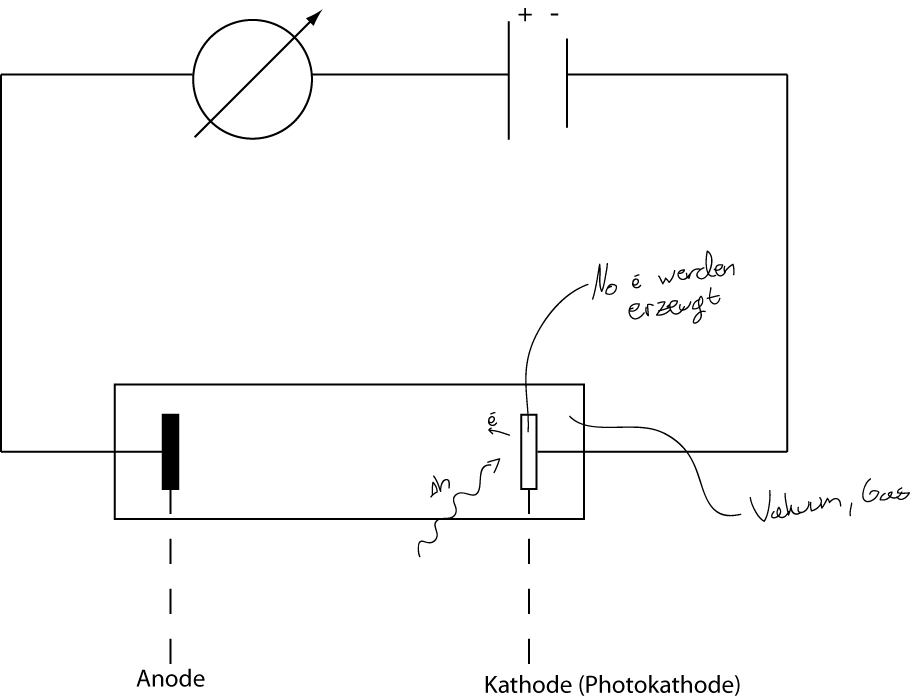
\includegraphics[width=0.8\linewidth]{skizzen/15/VL07/VL7_3}
	\\
	(i) \underline{Unselbstständige Gasentladung} \\
	\begin{center}
		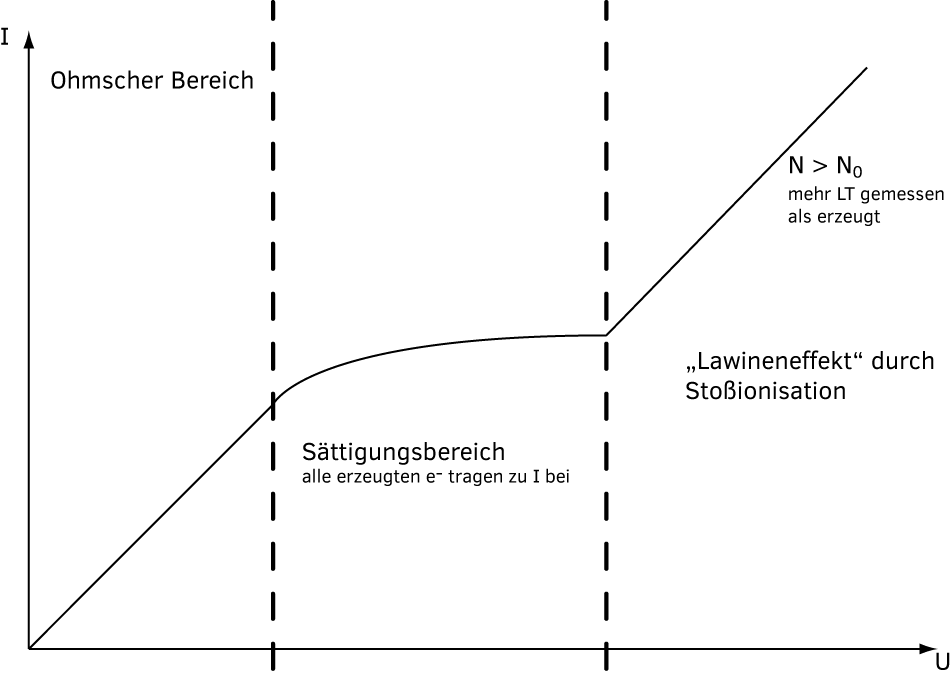
\includegraphics[width=0.8\linewidth]{skizzen/15/VL07/VL7_2}
	\end{center}
	\begin{center}
		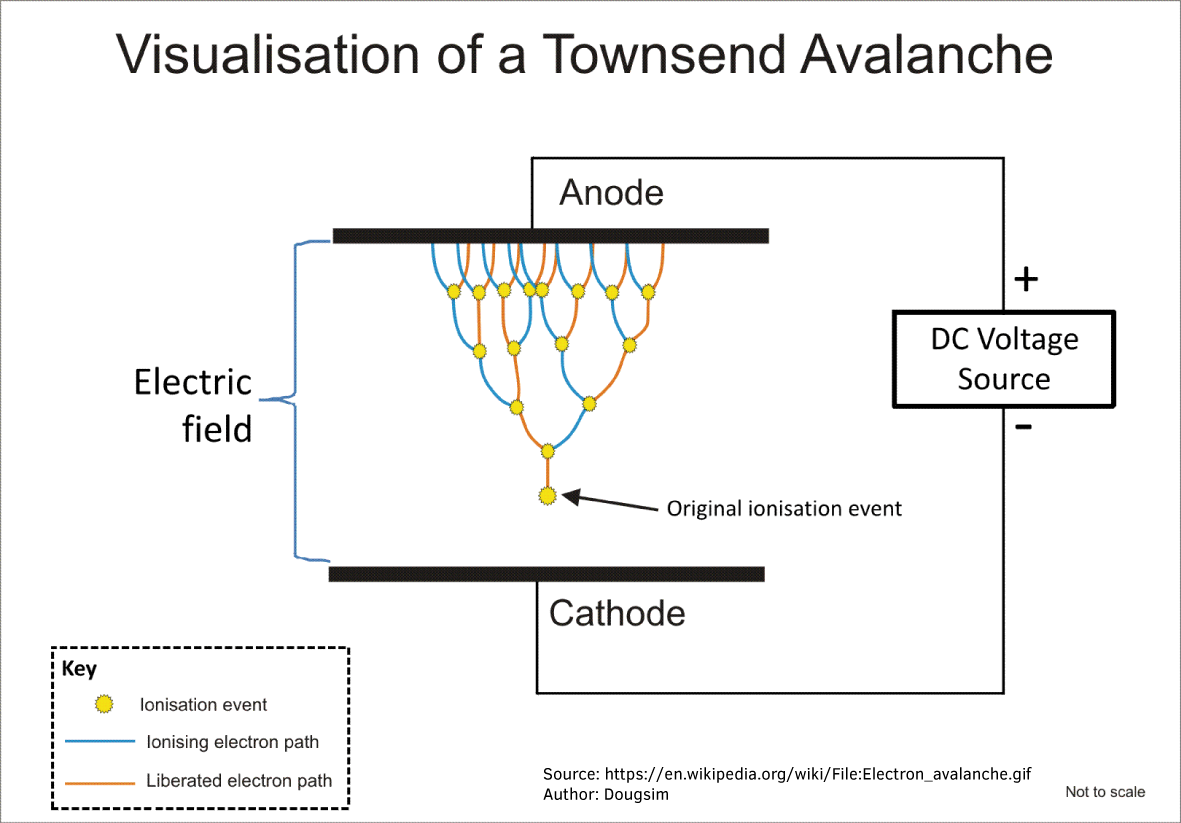
\includegraphics[width=0.7\linewidth]{skizzen/15/VL07/7}\\
		\begin{flushleft}
			Spannung ist sehr groß, Elektronen werden start beschleunigt, hohe Elektronenenergie Stoßionisation: \textbf{Lawineneffekt}\\
			\hfill \\
			Strom wird unabhängig von Zahl der Ionisation generierten Ladungsträger. 
		\end{flushleft}
	\end{center}
	$ \Rightarrow $ 1 Strompuls pro Ionisierungsereignis oder pro asgelöstem $ e^- $ ! \\
	$ \Rightarrow $ \underline{Selbstständige Gasentladung}
	\begin{itemize}
		\item \underline{Aufrechterhaltung} der Entladung ohne äußeren Einsatz!
		\item Voraussetzung: Hohe kinetische Energie ($ \longrightarrow $ hohe Spannung!)
		\item Häufig auch Lichtemission (Rekombination von $ e^- $ und Ion oder Relaxation angeregter Zustände)
		\item UV-Emission in Plasmen und in Leuchtstoffröhren genutzt
	\end{itemize}
%	\includegraphics[width=0.7\linewidth]{Skizzen/VL07/8}

	\subsection{Leistungsumsetzung beim Ladungstransport}
	\begin{itemize}
		\item Elektrolyte: Ladungstransport durch Ionen.
		\item Ladungstransport durch Elektronen: Stöße mit Gitterionen
	\end{itemize}
	Elektrische Energie $ \longrightarrow $ $ E_{kin} $ + Wärmeenergie.\\
	Leistung im Ohmschen Widerstand \emph{R} :\\
	\begin{center}
		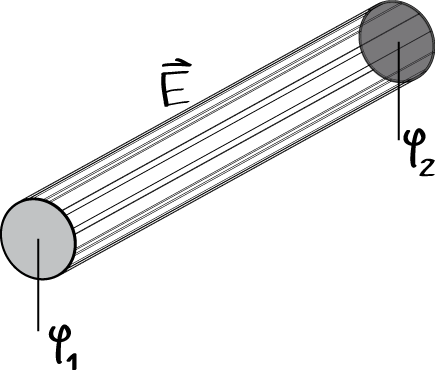
\includegraphics[width=0.4\linewidth]{skizzen/15/15_4-6/15_4B0}
	\end{center}

	\begin{align*}
	U = \varphi_2-\varphi_1,\hspace{5mm} W&=\int \vec{F} \cdot d\vec{r} = q \int\vec{E}d\vec{r} = \int q dU = U\cdot q  \\
	\text{Bei \emph{N} Ladungen: } W&=NUq=UQ  \\
	\end{align*}
	
	\begin{align*}
	\text{Leistung } &\text{ }P = \frac{dW}{dt} = \frac{dQ}{dt}U = I \cdot U \hspace{1cm} | (U=R\cdot I) \\
	\Rightarrow &\boxed{P = I^2R=\frac{1}{R} U^2 } \hspace{2mm} \text{[$ P $]}=\si{\watt}=\si{\volt\ampere}
	\end{align*}
	\paragraph{Anwendung:}
	- Elektrisch Betriebene Heizung \\
	Exp: $ \longrightarrow $ Hitzdrahtmesswerk 
	
	\subsection{Widerstandnetzwerke und Kirchhoffsche Regeln}
	
	\begin{itemize}
		\item Netzwerk: Leitsystem, in das Bauelemente eingefügt sind
		\item Hier nur Verbindungen von Widerständen und Stromquellen
		\item Alle Elemente: 2 Pole $ \longrightarrow $ 2 Anschlüsse \\
		Widerstände: passive 2 Pole, Stromquellen: aktive 2 Pole
		\item Richtungen/Vorzeichen: Strompfeile: geben formal Richtung positiver Ladungsträger an. \\
		passiv: $ + \longrightarrow - $ \hspace{1cm} aktiv: $ - \longrightarrow + $ \\
		Spannungspfeile: $ + \longrightarrow - $
	\end{itemize}
	\begin{center}
		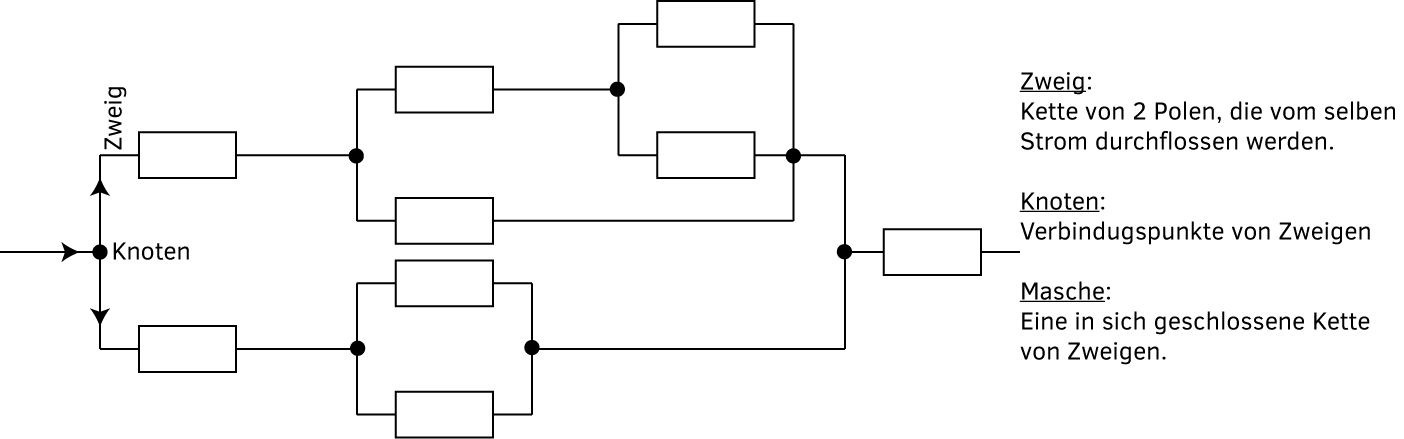
\includegraphics[width=1\linewidth]{skizzen/15/15_4-6/15_5B0}
	\end{center}

	$ \longrightarrow $ Ersetzen durch 1 Ersatzwiderstand
	
	\subsubsection{Kirchhoffsche Regeln}
	$ \longrightarrow $ Verallgemeinerung des Ohmschen Gesetzes, dass zu Gleichungssystem führt, mit dem immer alle unbekannten Ströme und Spannungen berechnet werden können. (G.R. Kirchhoff: 1845 (1824-1887))
	\begin{enumerate}
		\item Kontenregeln \\
		In einem Knoten kann keine Ladung gespeichert werden. \\
		$ \sum $Zufließende Ströme = $ \sum $Abfließende Ströme\\
		$ \sum_j I_j=0$ \hspace{1cm} ($ \forall $Knoten und "folgt" aus der Ladungserhaltung)
		\item Maschenregel \\
		Spannungen sind Potenzialdifferenzen. Für Maschen ohne elektromotorische Kraft gilt: \\
		In Masche: $ 0=\sum_j uj = \sum_j R_jU_j  $ (Umlaufspannung $ =0 $!)\\
	\end{enumerate}
	
	\begin{minipage}{\textwidth}
	\paragraph{Beispiel:} \hfill \\
	\begin{center}
		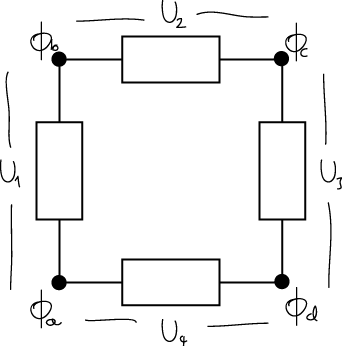
\includegraphics[width=0.4\linewidth]{skizzen/15/15_4-6/15_5B1}
	\end{center}
	

	\begin{align*}
	&U_1 = \phi_b - \phi_a \hspace{1cm} & U_3 = \phi_d - \phi_c \\
	&U_2 = \phi_c - \phi_d \hspace{1cm} & U_4 = \phi_a - \phi_d \\
	&{\displaystyle\sum_{j=1}^{4} Uj} = 0
	\end{align*}
	\end{minipage}
	\break
	
	\noindent Mit diesen Regeln lassen sich die Ströme  I Spannungen in einem beliebigen Netzwerk durch ein Gleichungssystem berechnen.
	
	\subsubsection{Serien-(Reihen)schaltung von Widerständen}
	\begin{center}
		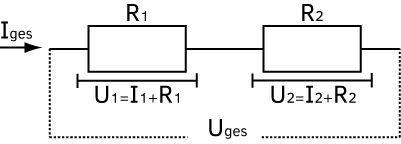
\includegraphics[width=0.5\linewidth]{skizzen/15/15_4-6/15_5B2}
	\end{center}
	 \noindent
	\begin{align*}
		&U_{ges} = U_1 + U_2 \\
		&I_1R_1+I_2R_2=I_{ges}R_{ges} \\
		&I_1=I_2=I_{ges} \Rightarrow \boxed{R_1+R_2=R_{ges}}
	\end{align*}

	\subsubsection{Parallelschaltung}
	\begin{center}
		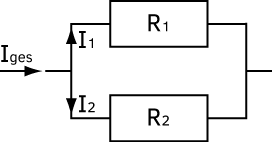
\includegraphics[width=0.5\linewidth]{skizzen/15/15_4-6/15_5B3}
	\end{center}
	\noindent
	\begin{align*}
		&U_{ges} = U_1 = U_2 && \\
		&I_{ges} = I_1 + I_2 &&\Rightarrow \frac{U_{ges}}{R_{ges}} = \frac{U_1}{R_1} + \frac{U_2}{R_2} \hspace{5mm} |\cdot U_{ges}^{-1} \\
		& &&\Rightarrow \boxed{\frac{1}{R_{ges}} = \frac{1}{R_1} + \frac{1}{R_2} } 
	\end{align*}
	
	\subsubsection{Beispiel} : Wheatstonesche Messbrücke
	\begin{center}
		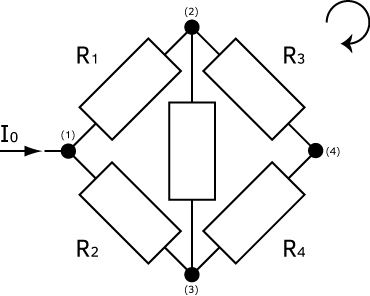
\includegraphics[width=0.5\linewidth]{skizzen/15/15_4-6/15_5B4}
	\end{center}
	\begin{math}
		\text{KR:} \\
		\text{(1): } I_0 = I_1 + I_2 \hspace{1cm} \text{(3): } I_4 = I_2 + I_5\\
		\text{(2): } I_1 = I_3 + I_5 \\
		\hfill \\
		\text{MR: } \\
		\text{\emph{l}: } I_1R_1+I_5R_5-I_2R_2=0 \\
		\text{\emph{r}: } I_3R_3+I_4R_4-I_5R_5=0 
	\end{math}
	$ \Rightarrow $ 5 Bestimmungsgleichungen für $ I_1,...,I_5 $ \\
	Bei Vorgabe von $ I_0 $ ist dieses Problem lösbar \\
	"$ \Rightarrow $" Durch Veränderung von $ R_2 $ und $ R_4 $ kann erreicht werden, dass $ I_5=0 $.\\
	Dies kann genutzt werden um Widerstände zu Messen.\\
	\begin{math}
		I_5 \overset{!}{=} 0 \Rightarrow I_1 = I_3,\hspace{2mm} I_2 = I_4 \\
		\overset{MR}{\Rightarrow} I_1 R_1 = I_2 R_2,\hspace{2mm} I_3 R_3 = I_4 R_4 \Rightarrow I_1 R_3 = I_2 R_4 \\
		\Rightarrow \frac{R_1}{R_3} = \frac{R_2}{R_4} \Rightarrow \text{ermittel } R_1
	\end{math}

	
	\subsection{Stromquellen, elektromotorische Kraft, Urspannung, Klemmspannung}
				

\end{document}
